\section[Desenvolvimento do Projeto]{Desenvolvimento do Projeto}
Esta seção tem como principal objetivo detalhar os artefatos utilizados pela equipe durante o período de construção do projeto. Desse modo, encontram-se descritos a seguir: o repositório do código fonte do projeto, o banco de dados utilizado, a arquitetura utilizada, os protótipos das telas desenvolvidas e as tecnologias utilizadas.

\subsection{Repositório do Código Fonte do Projeto}
O reposotório responsável por armazenar e manter o controle de versão do código fonte do projeto, encontra-se disponível para consulta por meio do link a seguir:
   \href{https://tools.ages.pucrs.br/o-turismo-rural-em-s-o-francisco-de-paula}{\textit{Repositório do Código Fonte}}

\subsection{Banco de Dados Utilizado}
  O sistema de gerenciamento de banco de dados utilizado para armazenar os dados referentes às atrações turísticas cadastradas e às informações de um contribuidor  foi MySQL \cite{MySQL}, que oferece recursos usando SQL. Mais informações estão disponíveis clicando aqui:
  \href{https://tools.ages.pucrs.br/o-turismo-rural-em-s-o-francisco-de-paula/wiki/-/wikis/Banco%20de%20Dados}{\textit{Banco de Dados}}

\begin{figure}[H]
    \centering
    \small
    \caption{Diagrama lógico do banco de dados do Turismo Rural}
    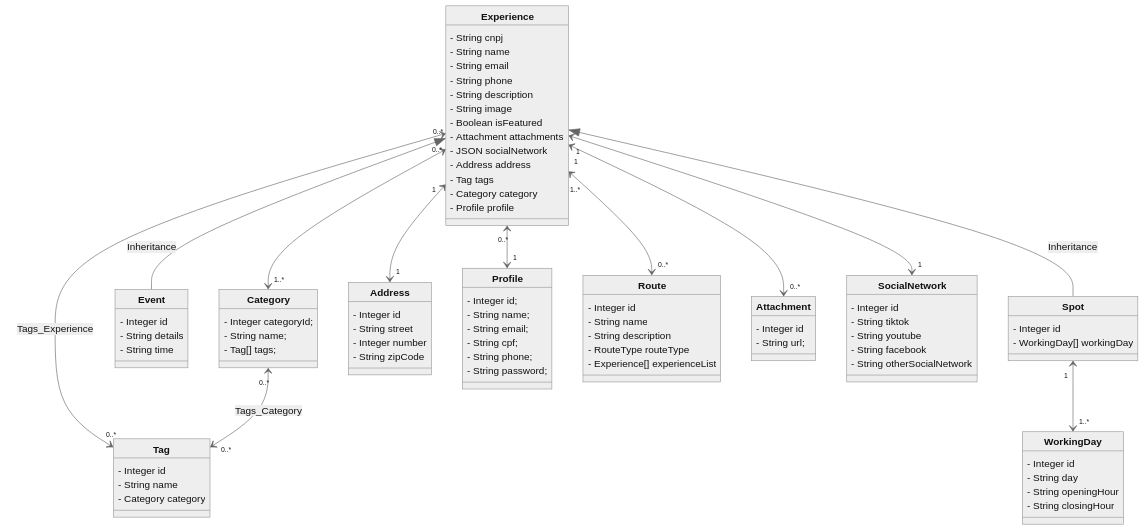
\includegraphics[width=0.9\linewidth]{conteudo/2 - ages I/conteudo/figures/bd_diagrama_logico.png}\\
    \label{fig:tr-bd-diagrama-logico}
    \begin{minipage}{0.95\linewidth}
    \raggedright
    \href{https://tools.ages.pucrs.br/o-turismo-rural-em-s-o-francisco-de-paula/wiki/-/wikis/Banco%20de%20Dados}{\textit{Fonte: https://tools.ages.pucrs.br/o-turismo-rural-em-s-o-francisco-de-paula/wiki/-/wikis/Banco\%20de\%20Dados}}
    \end{minipage}
\end{figure}

\subsection{Arquitetura Utilizada}
  A arquitetura escolhida para o desenvolvimento da aplicação consiste em uma API para comunicação entre \textit{frontend} e \textit{backend}. Já para o gerenciamento do banco de dados, optou-se por usar um container no Docker para executar o MySQL, utilizando  uma instância \ac{ec2} da \ac{aws} para hospedar e executar os diferentes componentes do sistema e \ac{s3} para o armazenamento de imagens. Mais informações podem ser encontradas aqui:
  \href{https://tools.ages.pucrs.br/o-turismo-rural-em-s-o-francisco-de-paula/wiki/-/wikis/arquitetura}{\textit{Arquitetura}}

\begin{figure}[H]
    \centering
    \small
    \caption{Diagrama de \textit{deploy} da infraestrutura do Turismo Rural}
    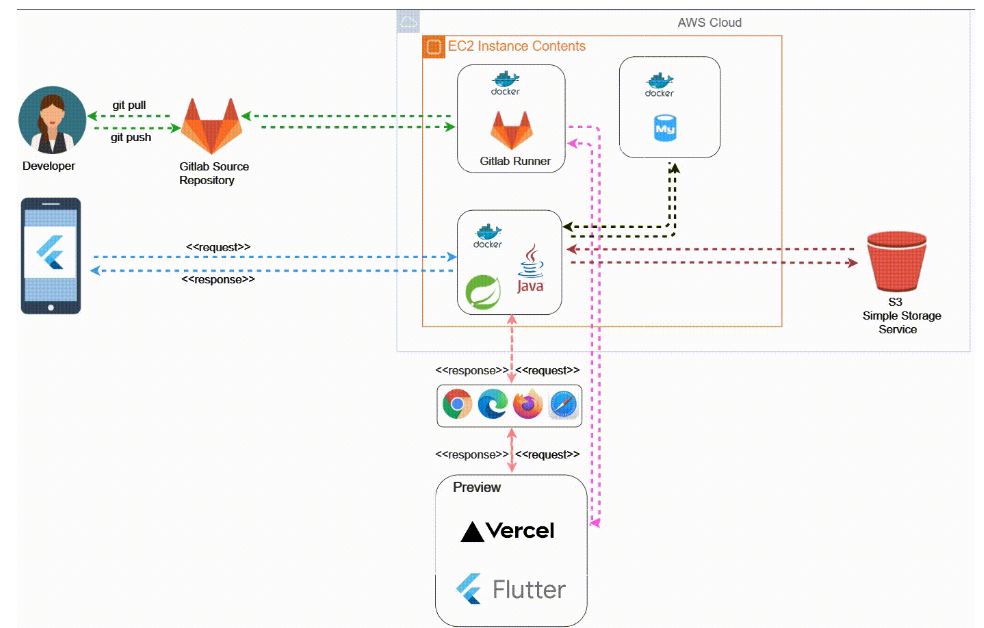
\includegraphics[width=0.9\linewidth]{conteudo/2 - ages I/conteudo/figures/diagrama_de_deploy.png}\\
    \label{fig:tr-diagrama-deploy}
    \begin{minipage}{0.95\linewidth}
    \raggedright
    \href{https://tools.ages.pucrs.br/o-turismo-rural-em-s-o-francisco-de-paula/wiki/-/wikis/arquitetura}{\textit{Fonte: https://tools.ages.pucrs.br/o-turismo-rural-em-s-o-francisco-de-paula/wiki/-/wikis/arquitetura}}
    \end{minipage}
\end{figure}

\subsection{Protótipos das Telas Desenvolvidas}
  Os protótipos das telas desenvolvidas, construídos utilizando a plataforma Figma, estão disponíveis para visualização ao clicar em:
  \href{https://tools.ages.pucrs.br/o-turismo-rural-em-s-o-francisco-de-paula/wiki/-/wikis/design}{\textit{Protótipo das Telas}}

\begin{figure}[H]
    \centering
    \small
    \caption{Protótipos das telas de boas-vindas, login e principal do Turismo Rural}
    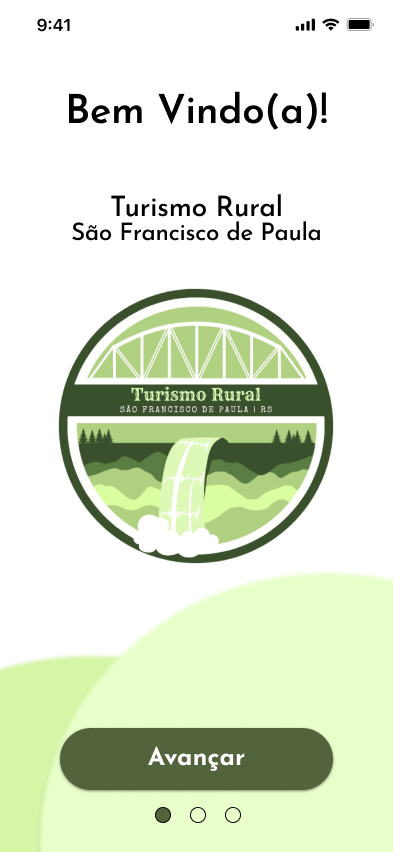
\includegraphics[width=0.31\linewidth]{conteudo/2 - ages I/conteudo/figures/bem_vindo.png}\hfill
    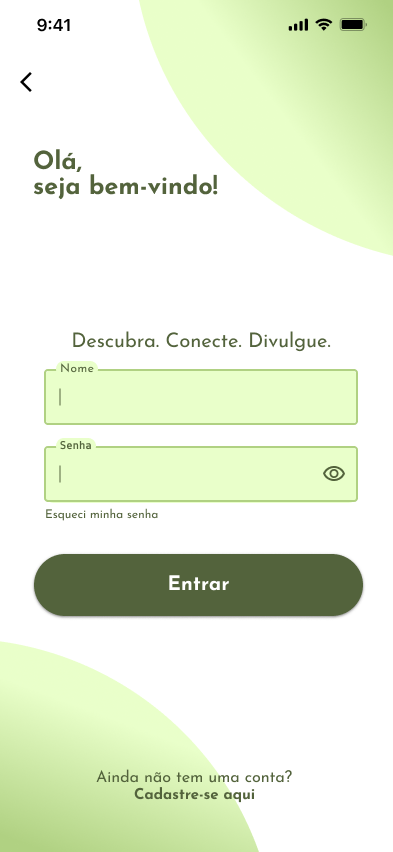
\includegraphics[width=0.31\linewidth]{conteudo/2 - ages I/conteudo/figures/login.png}\hfill
    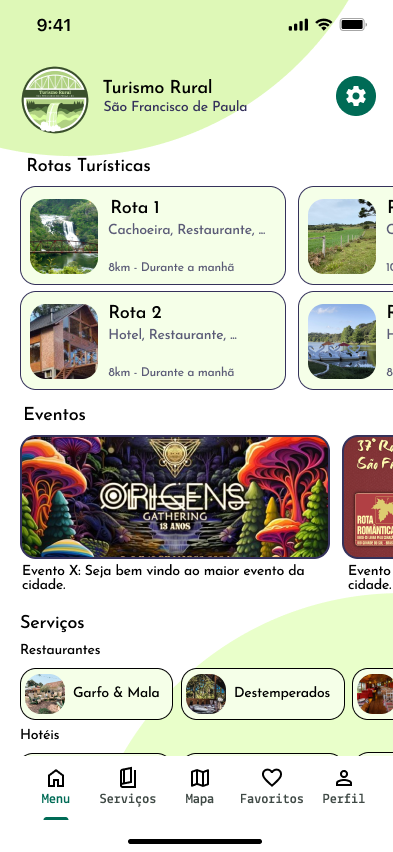
\includegraphics[width=0.31\linewidth]{conteudo/2 - ages I/conteudo/figures/tela_principal.png}\\
    \label{fig:tr-mockups}
    \begin{minipage}{0.95\linewidth}
    \raggedright
    \href{https://tools.ages.pucrs.br/o-turismo-rural-em-s-o-francisco-de-paula/wiki/-/wikis/design}{\textit{Fonte: https://tools.ages.pucrs.br/o-turismo-rural-em-s-o-francisco-de-paula/wiki/-/wikis/design}}
    \end{minipage}
\end{figure}

\subsection{Tecnologias Utilizadas}
Quanto às tecnologias utilizadas, para a parte do \textit{frontend} (desenvolvimento das telas) a equipe decidiu por trabalhar com a linguagem Dart \cite{Dart} e o \textit{framework} Flutter \cite{Flutter}; já para o \textit{backend}, optou-se por desenvolver em Java \cite{Java}; para o banco de dados, o sistema de gerenciamento escolhido foi MySQL; por fim, ainda foi feito uso de uma tecnologia denominada Vercel \cite{Vercel} para possibilitar o preview do projeto. Informações específicas de cada tecnologia podem ser encontradas em: 
\href{https://tools.ages.pucrs.br/o-turismo-rural-em-s-o-francisco-de-paula/wiki/-/wikis/arquitetura#tecnologias}{\textit{Tecnologias}}

